% 本论文基于 latexstudio/chinesejournal 的 cjc 文档类，依比赛要求适配。
% 上游作者 Zeping Lee；LPPL 1.3c 或更高版本，见同目录 LICENSE 与 cjc.dtx。
\documentclass{mathorcup-journal}
\usepackage{longtable,booktabs,array,hyperref,listings,xcolor}
\geometry{left=2cm,right=2cm,top=2.6cm,bottom=2.6cm}
\setlength{\columnsep}{0.75cm}
\setlength{\columnseprule}{0pt}
\setlength{\tabcolsep}{2pt}
\IfFontExistsTF{LXGW WenKai GB Lite}{\setmonofont{LXGW WenKai GB Lite}}{\setmonofont{Arial Unicode MS}}
% 赛规：匿名、无页眉、正文页脚居中。
\fancypagestyle{contest}{\fancyhf{}\renewcommand{\headrulewidth}{0pt}\fancyfoot[C]{\thepage}}
\fancypagestyle{plain}{\fancyhf{}\renewcommand{\headrulewidth}{0pt}\fancyfoot[C]{\thepage}}
\pagestyle{contest}
\setlength{\parindent}{2em}
\setlength{\parskip}{0.3em}
\setlength{\emergencystretch}{3em}
\hypersetup{hidelinks}
\lstset{basicstyle=\ttfamily\tiny,breaklines=true,breakatwhitespace=false,breakautoindent=false,breakindent=0pt,columns=fixed,keepspaces=true,numbers=left,numberstyle=\tiny,frame=single,literate={_}{{\char95\allowbreak}}1}
\begin{document}
\twocolumn[{\begin{center}{\zihao{2}\heiti 基于原始感官评分与缺陷约束的啤酒风味预测和风格迁移}\end{center}\vspace{1.2em}
\noindent\textbf{摘\quad 要}\quad 针对啤酒感官分级、关键化合物识别和风格迁移问题，本文结合竞赛附件与公开的逐人感官评分，建立从评分重建到迁移可行性分析的研究流程。首先核查250款啤酒的样本对应关系，利用2197条原始评分构造各感官属性的0—6分面板均分和七级评分分布。以啤酒为单位进行三折五次重复验证，极端随机树与梯度提升树的等权融合在30个Aroma/Flavour核心属性上的均分预测平均绝对误差为0.50222，在全部50项上的误差为0.43560；核心属性的风格中位数基线误差为0.50969，二者差值的固定预测条件下95\%重采样区间为[-0.01914，0.00418]。七级分布模型在核心属性上的累计分布平方距离为0.02178，对应的个人评分期望RPS为0.11044；核心属性的面板众数一致率为80.52\%，非零众数一致率为24.33\%。其次，构建化合物相关图并比较图约束与普通岭回归：真实图的单折平均误差为0.537035，无图为0.536911；按酒聚合重复预测后分别为0.524865和0.526148。最终因素模型选择图惩罚系数0，150条Top-3结果中36条满足描述性支持条件。最后，对Tripel、Kriek和Lambic生成风味谱，并在冻结候选后进行独立角色复核；真实留出来源的10条重复迁移记录涉及7款酒，其中1条满足全部代理条件。浓度域混配在四项浓度均不增加的严格约束下，对55条来源与划分记录均未找到正的目标风格份额；改用阈值超额不增加的化学风险约束后，参考阈值下30条记录允许正份额。研究结果为感官预测、因素解释及迁移约束设计提供了可复核的定量依据。

\noindent\textbf{关键词}\quad 啤酒风味；感官评分；有序分布；化合物相关网络；风格迁移；缺陷约束
\vspace{1.5em}}]
\thispagestyle{empty}
\clearpage
\onecolumn
\tableofcontents
\thispagestyle{empty}
\twocolumn
\setcounter{page}{1}
\section{问题分析}

啤酒风味由挥发性化合物、理化条件及其相互作用共同影响。题目要求完成三项任务：根据化合物数据预测0—6分的感官等级；利用化合物相关关系识别各感官维度的三个关键因素，并论证稳定性和化学合理性；在给定风格下生成化合物谱与感官画像，研究Pils/Lager向Tripel的迁移及缺陷控制。


题面描述数据约226款酒、Aroma和Flavour合计约40项；实际用于建模的附件包含250款酒、231个数值输入和50个感官目标，其中Aroma与Flavour前缀各15项。本文对全部50项目标建模与输出，同时单独报告30个Aroma/Flavour核心属性。原始个人评分来自作者公开数据[1][2]，附件中的标准化分值用于样本对应核查，不作为0—6分值直接使用。


三问共用同一数据与验证框架。第一问分别建立面板均分和个人评分分布模型；第二问将训练折内的化合物网络引入多目标回归，并以无图和打乱图作对照；第三问将生成、候选搜索、代理评价和浓度域可行性分析依次连接。各方法基于极端随机树、梯度提升、岭回归、图正则化和保形预测等已有方法[3][4][5][6][7]，本文的工作重点是将这些方法与题目的评分尺度、缺陷约束和验证条件对应起来。


\section{数据处理与评分端点}

\subsection{样本与字段核查}

附件1包含250行、234列，其中3列为样本元信息；附件4包含250行、53列。两表按唯一的beer字段对齐，并核对风格标签。评分卡与监督表中存在命名差异，例如A/F\_ester\_fruity对应A/F\_esters\_fruity，4vg对应X4vg。评分卡的乙醛Aroma/Flavour位置没有独立监督列，Barnyard汇总公式存在疑似引用偏差，相关字段按原始记录保留。


将附件2的相关矩阵与附件1重算结果比较，矩阵与Spearman秩相关的平均绝对差约为1.58×$10^{-16}$，与Pearson相关的平均绝对差约为0.0873。因此，本文将附件2解释为秩相关矩阵。对建模输入，所有截尾界限、中位数和标准化参数均只由训练数据估计；测试样本使用对应训练参数变换。部分化合物字段为对数浓度，负值可对应小于1的原始浓度。


\subsection{原始评分对应与人员权重}

作者公开数据含2197条逐人评分、16名匿名评分人员和250款啤酒，评分取值为0—6。根据公开补充表行序建立原始编号与附件beer的对应关系，再把50个属性分成互不重叠的两组进行一对一匹配核查，两组结果均与行序对应一致。38个无人员内零方差问题的属性重现公开连续标签，最大误差为2.8×$10^{-8}$；其余12项涉及零方差，采用部分样本估计替代常数并在其余样本上核验。该对应关系用于数据整合，预测测试集仍按啤酒划分。


同一人员对同一款酒的重复评分先取均值，再对人员等权平均。记第$b$款酒、第$j$个属性中人员$t$的第$r$次评分为$s_{btrj}$，则面板均分为


\begin{equation}
\bar s_{bj}=\frac{1}{|T_b|}\sum_{t\in T_b}\frac{1}{n_{bt}}\sum_{r=1}^{n_{bt}}s_{btrj}.
\end{equation}

每款酒对应3—14名不同人员。采用相同的人员权重，七级评分分布定义为


\begin{equation}
q_{bjk}=\frac{1}{|T_b|}\sum_{t\in T_b}\frac{1}{n_{bt}}\sum_{r=1}^{n_{bt}}\mathbf1(s_{btrj}=k),\quad k=0,\ldots,6.
\end{equation}

面板均分、个人评分分布和面板众数分别描述平均强度、评分离散情况和最常见等级。后续预测和评价保持这三种端点的区别。


\subsection{化学尺度与异常}

公开校准化学表提供70个数值参考字段。比较恒等、半最小正值替换及替换后取常用对数等规则后，38列在全部可比记录中一致；其余32列存在80处数值差异，保留供敏感性分析。DMS和4VG的零值采用半最小正值替换后可重现对应变换，该规则的仪器检出限尚未取得。


浓度混配分析选用来源标注单位为mg/L、g/L、$\mu$g/L或体积分数的61个字段。五个综合量的13种候选重算公式均未达到预设重现精度，故条件生成模型排除这五个综合量，使用226个非综合字段。浓度单位与历史来源可以追踪，但完整标准曲线、回收率及新批次测量信息仍需补充。


\section{第一问：感官等级与面板均分预测}

\subsection{七级分布与评价指标}

以式（2）的七级分布为监督目标，使用多输出极端随机树估计各等级概率$\hat p_{bjk}$。预测众数用于精确等级决策，预测中位数用于绝对等级损失决策：


\begin{equation}
\begin{aligned}\hat g_{\mathrm{mode}}=\arg\max_k\hat p_k,\\
\hat g_{\mathrm{med}}=\min\left\{k:\sum_{h=0}^{k}\hat p_h\ge 0.5\right\}.\end{aligned}
\end{equation}

记预测与观测分布在等级边界$k$的累计概率为$P_k$和$Q_k$，累计分布平方距离定义为


\begin{equation}
D=\frac{1}{6}\sum_{k=0}^{5}(P_k-Q_k)^2.
\end{equation}

该指标衡量预测分布与历史面板经验分布之间的距离。对个人实际等级$Y$计算的标准有序概率评分为$\mathrm{RPS}(P,Y)=\frac16\sum_{k=0}^{5}(P_k-\mathbf1(Y\le k))^2$[8]。按经验分布取期望后有


\begin{equation}
\mathbb E_{Y\sim q}[\mathrm{RPS}(P,Y)]=D+\frac16\sum_{k=0}^{5}Q_k(1-Q_k).
\end{equation}

式（5）的第二项反映面板评分分歧，因此分布距离和个人期望RPS需要分别报告。面板众数一致率以每款酒的预测众数与观测面板众数是否相同计算；非零众数一致率仅在观测面板众数大于0的记录上计算。各方法的核心属性结果见表1和图1，频率模型的等级混淆见图2。


\begin{table*}[t]
\centering\small\renewcommand{\arraystretch}{1.2}
\caption{核心属性七级分布模型的比较}
\begin{tabular}{>{\raggedright\arraybackslash}p{0.182\textwidth}>{\raggedright\arraybackslash}p{0.182\textwidth}>{\raggedright\arraybackslash}p{0.182\textwidth}>{\raggedright\arraybackslash}p{0.182\textwidth}>{\raggedright\arraybackslash}p{0.182\textwidth}}
\toprule
核心30项方法 & 累计分布平方距离$D$ & 个人期望RPS & 面板众数一致率 & 非零众数一致率 \\
\midrule
训练总体分布 & 0.02820 & 0.11685 & 79.31\% & 21.30\% \\
风格分布基线 & 0.02313 & 0.11179 & 80.72\% & 26.58\% \\
频率极端随机树 & 0.02178 & 0.11044 & 80.52\% & 24.33\% \\
累计概率极端随机树 & 0.02170 & 0.11036 & 80.65\% & 24.88\% \\
\bottomrule
\end{tabular}
\end{table*}

核心属性观测面板众数为0的比例为78.03\%。频率极端随机树相对总体分布基线的$D$下降22.74\%，个人期望RPS下降5.49\%；风格分布基线的非零众数一致率高于两种树模型。累计概率模型相对频率模型的核心$D$差值为-0.000081，固定预测条件下的95\%重采样区间为[-0.000169，0.000004]。现有证据支持报告各方法的差异，同时显示非零等级识别仍是主要改进方向。


核心30项的7500条啤酒—属性记录中，观测众数非零的记录为1648条，其中27.85\%被预测为0，24.33\%预测等级与观测众数完全一致。例如，A\_hops\_noble的49条非零众数记录全部预测为0，说明总体一致率会掩盖个别属性的识别困难。


针对零等级占比高的问题，进一步构造两阶段极端随机树：第一阶段估计0分概率$p_0$，第二阶段在训练集的非零评分上估计条件概率$r_k$，并以非零评分比例加权，组合得到$p_k=(1-p_0)r_k$。采用同一三折五次划分，并将两阶段模型中每个树模型的树数与频率模型均设为32。核心非零众数一致率由24.76\%增至25.49\%，增量为0.73个百分点，固定预测条件下的95\%重采样区间为[-0.91，2.30]个百分点；累计分布平方距离由0.02178增至0.02200。原200棵树频率模型的非零众数一致率为24.33\%。各模型树数相同不代表整体计算量相同；现有结果作为探索性对照，频率模型继续作为主要分布模型。


全部50项中，频率极端随机树的面板众数一致率为79.10\%，非零众数一致率为31.33\%；总体分布基线分别为77.84\%和26.92\%。生成的概率分布、众数和中位数结果按属性分别保存，以适配不同的决策损失。


\begin{figure*}[t]
\centering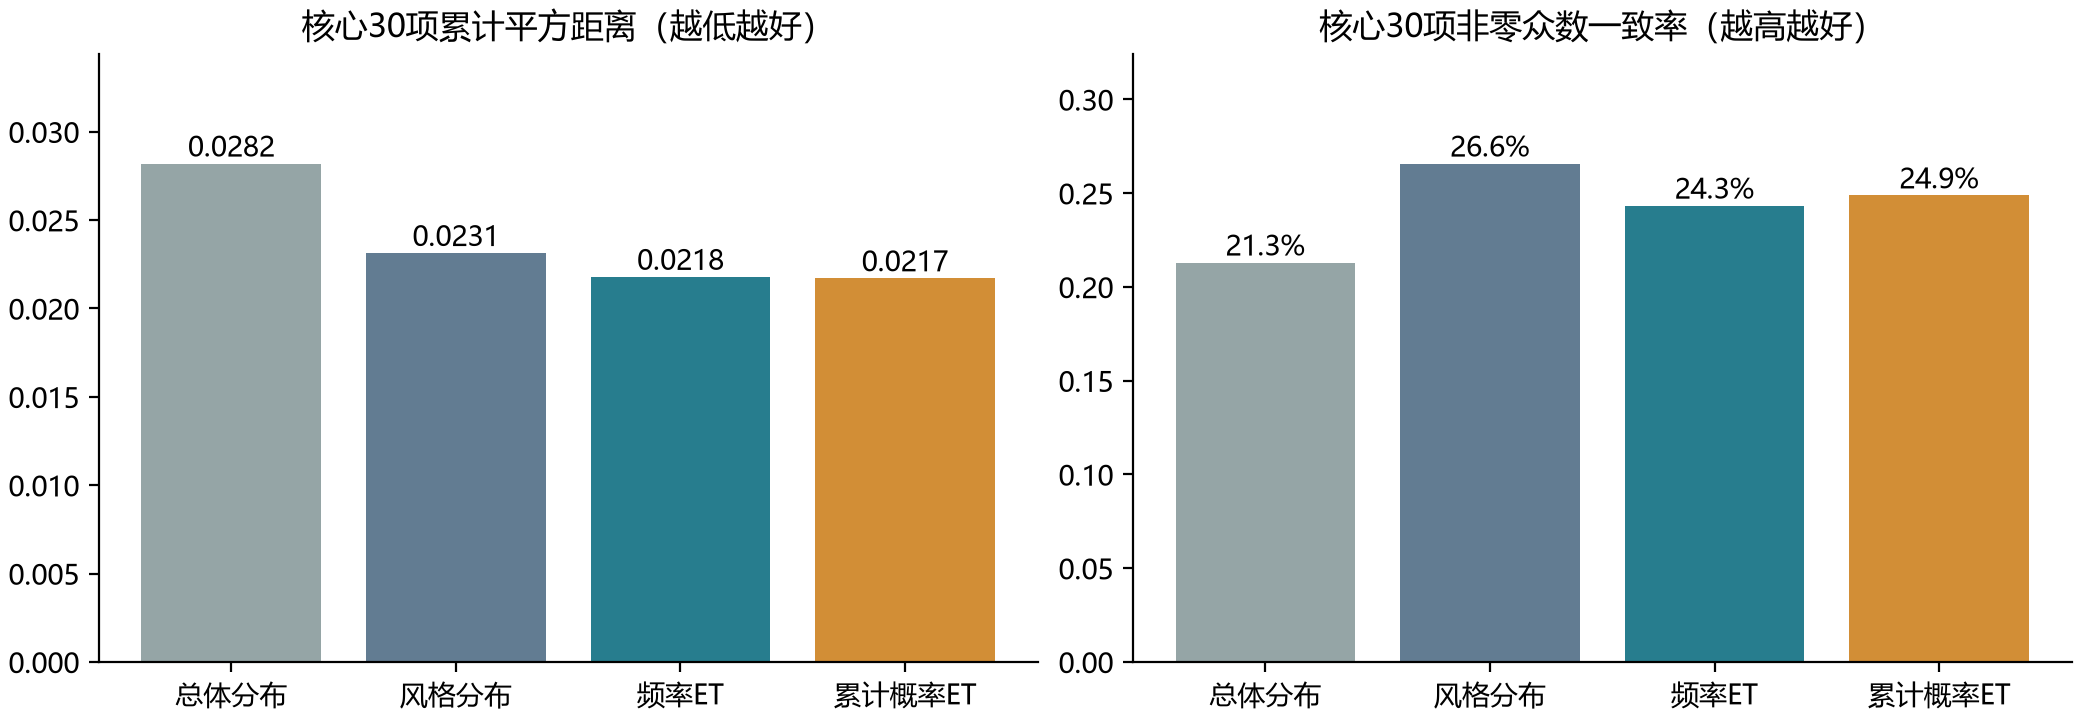
\includegraphics[width=0.95\textwidth]{figures/ordinal_review.png}
\caption{等级分布预测的累计距离与非零众数识别比较。}
\end{figure*}
\begin{figure}[t]
\centering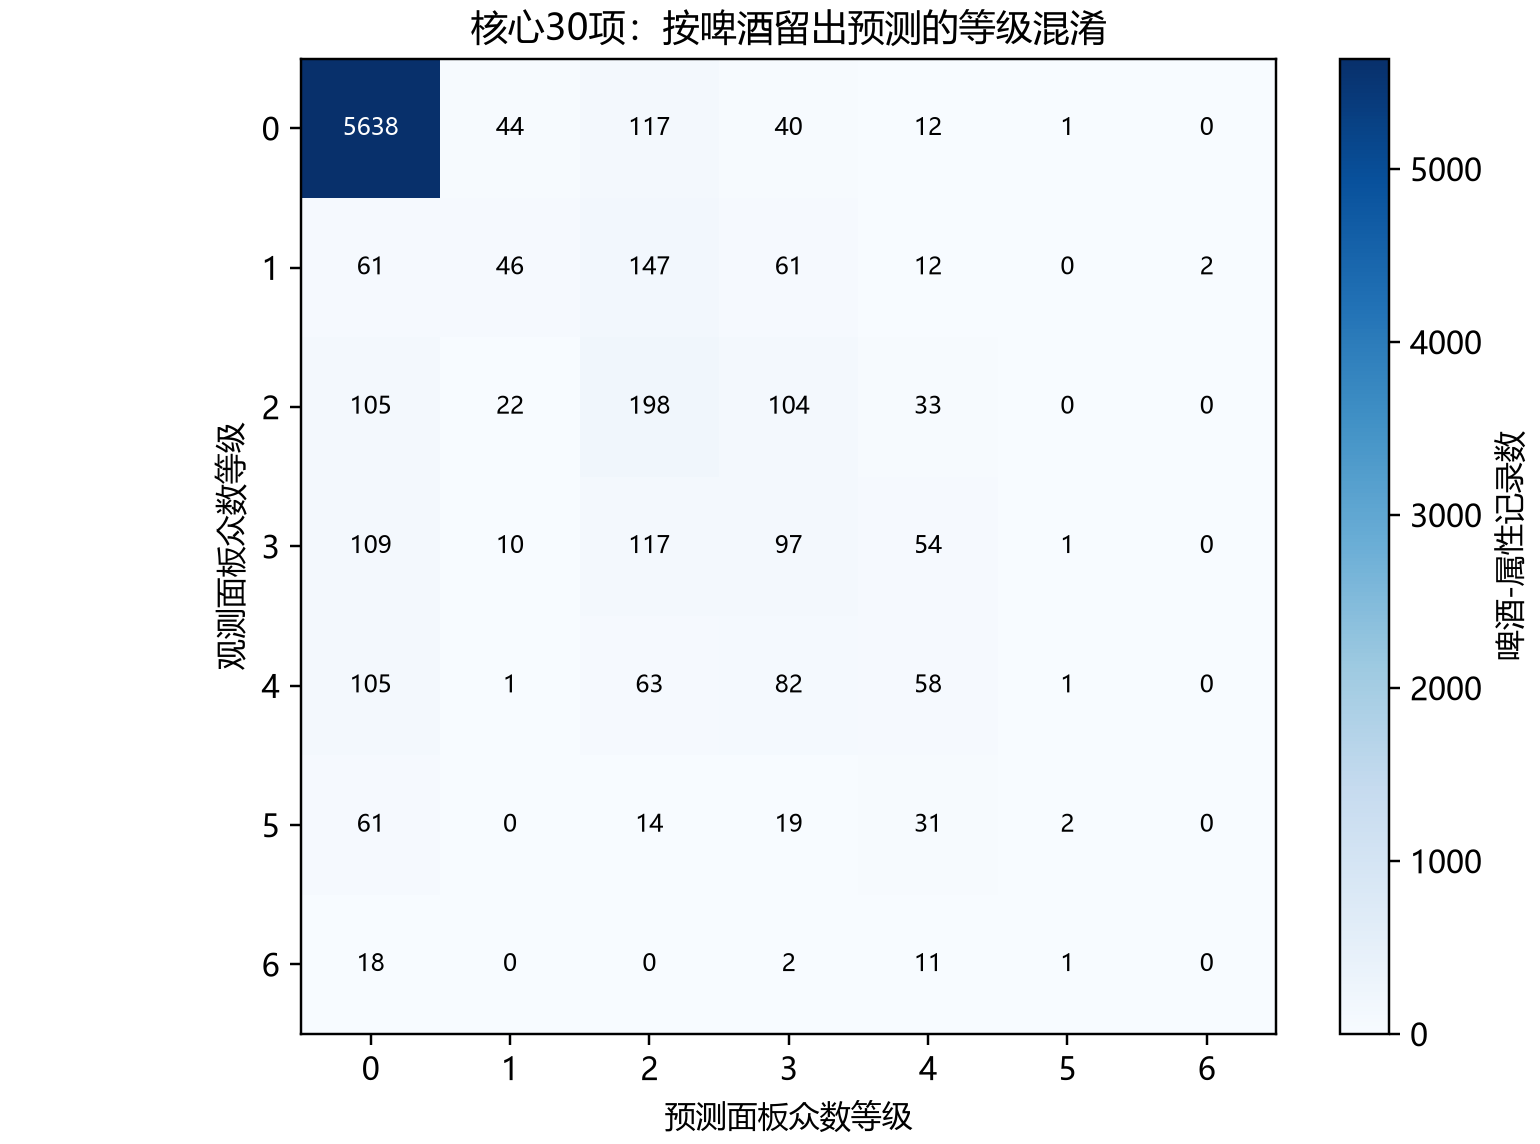
\includegraphics[width=0.95\columnwidth]{figures/ordinal_confusion.png}
\caption{核心30项留出预测的面板众数等级混淆。}
\end{figure}
\subsection{面板均分预测}

对面板均分，比较训练均值、训练中位数、风格中位数、岭回归、极端随机树、梯度提升树及固定等权融合。外层采用按风格分层的三折五次重复划分；对同一啤酒的五次留出预测取平均，再计算平均绝对误差。岭回归参数在训练数据内选择，其他方法使用预先固定的设置。结果见表2。


\begin{equation}
\mathrm{MAE}=\frac{1}{nq}\sum_{b=1}^{n}\sum_{j=1}^{q}|\bar s_{bj}-\hat s_{bj}|.
\end{equation}

\begin{table}[!h]
\centering\small\renewcommand{\arraystretch}{1.2}
\caption{面板均分预测误差比较}
\begin{tabular}{>{\raggedright\arraybackslash}p{0.290\columnwidth}>{\raggedright\arraybackslash}p{0.290\columnwidth}>{\raggedright\arraybackslash}p{0.290\columnwidth}}
\toprule
方法 & 核心30项MAE/分 & 全50项MAE/分 \\
\midrule
训练均值 & 0.60450 & 0.54879 \\
训练总体中位数 & 0.58785 & 0.52275 \\
风格中位数 & 0.50969 & 0.44712 \\
岭回归 & 0.52270 & 0.45708 \\
极端随机树 & 0.50589 & 0.44336 \\
梯度提升树 & 0.50819 & 0.43780 \\
固定等权融合 & 0.50222 & 0.43560 \\
\bottomrule
\end{tabular}
\end{table}

融合模型核心误差比训练均值低0.10228分，比风格中位数低0.00747分。以酒为单位、按风格分层，对固定的留出预测重采样5000次，融合与风格中位数的误差差值区间为[-0.01914，0.00418]；融合与极端随机树的差值为-0.00367，区间为[-0.00668，-0.00056]。这些区间反映当前留出预测的样本重采样变化，未纳入模型重训和选择过程的不确定性。风格中位数依赖已知风格标签，适合用于分析风格信息提供的基线。


\subsection{预测区间与缺失压力}

另用极端随机树进行五次分割保形实验，每次分别使用150款酒训练、50款校准、50款测试，按属性校准绝对残差。五次分割的逐属性平均覆盖率为90.06\%，平均区间宽度为1.7342分。覆盖率反映该实验中的逐维面板均分区间；不同属性存在差异，例如barnyard、F\_malt\_all和stale hops的平均覆盖率分别为84.0\%、84.8\%和85.2\%。


按历史面板人员数分组，3—4人组的描述性覆盖率为74.00\%，对应12款不同酒、750条重复测试的啤酒—属性记录；5—7人组为86.89\%，8人及以上组为92.94\%。分组测试中同一款酒可重复出现，且最小组样本有限，这些比例用于定位覆盖差异。


为考察输入缺失，测试阶段在原有缺失基础上增加0\%、5\%、10\%和20\%的随机缺失，使用训练阶段拟合的插补参数。该实验反映随机丢失输入的压力；低浓度未检出或整类检测通道缺失的影响，需要另设缺失机制实验。


\section{第二问：化合物图与关键因素}

\subsection{图构建和模型}

在全部数据上描述化合物相关结构时，取$|r|\ge 0.7$得到231个节点、109条边。模型验证时，每个训练折单独计算相关图。令$W$为带符号权重矩阵，$L=\operatorname{diag}(\sum_j|W_{ij}|)-W$，多目标系数矩阵$B$由下式估计：


\begin{equation}
\hat B=\arg\min_B\{\|Y_c-ZB\|_F^2+\alpha\|B\|_F^2+\lambda\operatorname{tr}(B^TLB)\}.
\end{equation}

对单个系数向量$b$，有$b^TLb=\sum_{i<j}|W_{ij}|(b_i-\operatorname{sign}(W_{ij})b_j)^2\ge0$。因此当$\alpha>0$且$\lambda\ge0$时，目标函数具有唯一解。正相关边鼓励系数接近，负相关边鼓励系数方向相反。$\alpha$、$\lambda$和相关阈值均在训练折内部选择；节点标签打乱图用于检验具体网络结构的作用。真实图与无图的比较见表3。


\begin{table}[!h]
\centering\small\renewcommand{\arraystretch}{1.2}
\caption{图模型两种评价口径的比较}
\begin{tabular}{>{\raggedright\arraybackslash}p{0.217\columnwidth}>{\raggedright\arraybackslash}p{0.217\columnwidth}>{\raggedright\arraybackslash}p{0.217\columnwidth}>{\raggedright\arraybackslash}p{0.217\columnwidth}}
\toprule
核心30项评价口径 & 无图MAE & 真实图MAE & 真实图减无图 \\
\midrule
15个留出折误差的平均 & 0.536911 & 0.537035 & +0.000124 \\
每酒五次预测平均后的误差 & 0.526148 & 0.524865 & -0.001283 \\
\bottomrule
\end{tabular}
\end{table}

两种口径分别衡量单次拟合与重复预测聚合后的误差，真实图的差异均较小。聚合口径下，以酒为单位的固定预测条件重采样差值区间为[-0.002392，-0.000177]。最终全数据描述模型选得$\lambda=0$，因此后续Top-3由岭回归系数确定。


\subsection{因素稳定性与化学解释}

对每个感官目标，按标准化输入的岭回归系数绝对值选取三个化合物或元素，共得到150条因素记录。采用200次以酒为单位的bootstrap，重新建立预处理与相关图，并保持全数据选定的参数；同时计算留出数据上的普通置换和风格内置换贡献。某因素被置换前后的误差增加量用于衡量该因素对预测的贡献。


描述性支持条件为：bootstrap入选频率至少0.5、至少在5个训练折入选，且所选折的普通与风格内置换平均贡献均为正。150条记录中有36条满足条件。该频率以固定参数为前提；重采样中重新选参可进一步评估完整选择流程的稳定性。


化学解释结合统计证据逐项给出。X4VG与4VG感官属性的关联，与4VG相关香气研究方向一致[9]；iron与金属感的关联，可结合金属诱发口腔氧化的研究讨论[10]；linalool与芫荽风味存在文献依据[11]，其当前入选频率低于0.5。对于A\_hops\_all的iron，风格中心化后的Top-3保留比例为0.1，说明其排名对风格差异敏感。相关性较强的化合物还会在模型中相互替代，因此完整因素表同时保留频率、置换贡献、单位和文献对应信息。


\section{第三问：风味生成与迁移可行性}

\subsection{风格条件生成}

以tasting\_category\_fine为风格标签，比较风格内重采样、局部凸组合、条件PCA高斯生成和受约束局部凸组合。每次分层划分设搜索训练集G为100款、评价训练集J为100款、真实留出集T为50款；对Tripel、Kriek、Lambic，每种方法在每次划分下生成40个谱。候选在G中形成并冻结，再由J模型复核；T用于检验留出来源的表现。


局部凸组合的形式为$x_{\mathrm{new}}=u x_a+(1-u)x_b$，其中$x_a,x_b$为同风格邻近样本，$0\le u\le1$。生成谱使用最大均值差异MMD、范围检查、复制比例和J风格分类结果评价[12]。对于Tripel，受约束局部凸组合的J目标风格识别率为69.5\%，高于风格内重采样的56.5\%；其MMD平方为0.1158，高于重采样的0.1034。分类识别率与分布距离反映不同性质，应结合覆盖度和重复率共同判断生成质量。已有MMD采用包含对角项的V统计量，结果受有限样本影响。


在冻结生成谱上，利用G和J分别训练的原始评分模型生成50项面板均分和整数等级画像。画像表示模型对化合物谱的预测；实际风味需通过制备和品评测量。


\subsection{冻结候选与代理复核}

迁移搜索限制特征变动半径、目标风格支持及四项化学缺陷字段，同时要求陈旧酒花感官代理不增加。在候选冻结后，补充使用G和J分别训练的原始评分尺度模型复核stale hops，候选及排序保持固定，复核结果见表4。


\begin{table*}[t]
\centering\small\renewcommand{\arraystretch}{1.2}
\caption{冻结迁移候选的代理复核结果}
\begin{tabular}{>{\raggedright\arraybackslash}p{0.303\textwidth}>{\raggedright\arraybackslash}p{0.303\textwidth}>{\raggedright\arraybackslash}p{0.303\textwidth}}
\toprule
半径为1的迁移记录 & 全部来源与划分：55条 & T留出来源：10条 \\
\midrule
G搜索可行 & 51 & 10 \\
原J代理支持 & 11 & 2 \\
同时满足新增G/J原始尺度stale hops条件 & 6 & 1 \\
\bottomrule
\end{tabular}
\end{table*}

T来源的10条记录涉及7款不同酒；重复划分形成的记录不是新增酒样。G和J的评分代理对部分候选给出不同判断，说明仅凭搜索模型的可行结果不足以确定迁移效果。


以第1次划分的来源酒81为例，半径1的冻结统计候选在G模型下的stale hops预测由0.8333降至0.3072，在J模型下由0.2629升至0.3098；该候选未获得原J代理支持。另一项浓度混配分析中，同一来源和划分在严格协议下的最大Tripel份额为0；参考阈值风险协议下，四项化学约束允许的最大份额为0.3514。这两项分析分别作用于统计候选和浓度域混配，前者展示评价模型分歧，后者展示约束定义对可行域的影响。


\subsection{严格浓度约束与阈值风险约束}

在61个报告浓度字段构成的次级分析中，以Pils来源酒和G中的Tripel锚点进行浓度域线性混配。设来源浓度为$c_s$、锚点浓度矩阵为$C_A$、锚点份额为$w$，则


\begin{equation}
c_{\mathrm{mix}}=(1-\mathbf1^Tw)c_s+C_Aw,\quad w\ge0,\quad\mathbf1^Tw\le0.75.
\end{equation}

协议A要求DMS、双乙酰、4VG和trans-2-nonenal四项浓度逐项不增加。令$D$为各锚点与来源在这四项上的浓度差，最大目标份额问题为


\begin{equation}
\max_w\ \mathbf1^Tw,\qquad Dw\le0,\quad w\ge0,\quad\mathbf1^Tw\le0.75.
\end{equation}

对55条来源与划分记录，协议A所得最大目标份额均为0。对各行按正尺度归一化得到$D_{\mathrm{norm}}$；若存在$v\ge0$，使$D_{\mathrm{norm}}^Tv$对每个锚点均严格为正，则任意非零$w\ge0$都有$v^TD_{\mathrm{norm}}w>0$，与协议A矛盾。55条记录均找到正余量证书，其中39条可由单项约束阻塞解释，16条需要联合约束。分别删除DMS、双乙酰、4VG和nonenal约束后，允许正份额的记录数为30、4、0和4；该消融用于定位阻塞来源，结果见图3。


题目强调超阈值缺陷，本文进一步设风险函数$R_d(c)=\max(c/t_d-1,0)$，以协议B要求$R_d(c'_d)\le R_d(c_d)$，等价于$c'_d\le\max(c_d,t_d)$。参考阈值取DMS 19 $\mu$g/L、双乙酰0.09 mg/L、4VG 0.2 mg/L、nonenal 0.1 $\mu$g/L[13][14]。以参考阈值的0.5、1和2倍计算时，55条记录中分别有15、30和34条允许正的Tripel份额。该结果仅检验四项化学风险约束；目标风格提升和stale hops仍需按冻结候选流程评价。阈值与啤酒基质、测量方法相关，零浓度记录还受到未知检出限影响。


\begin{figure*}[t]
\centering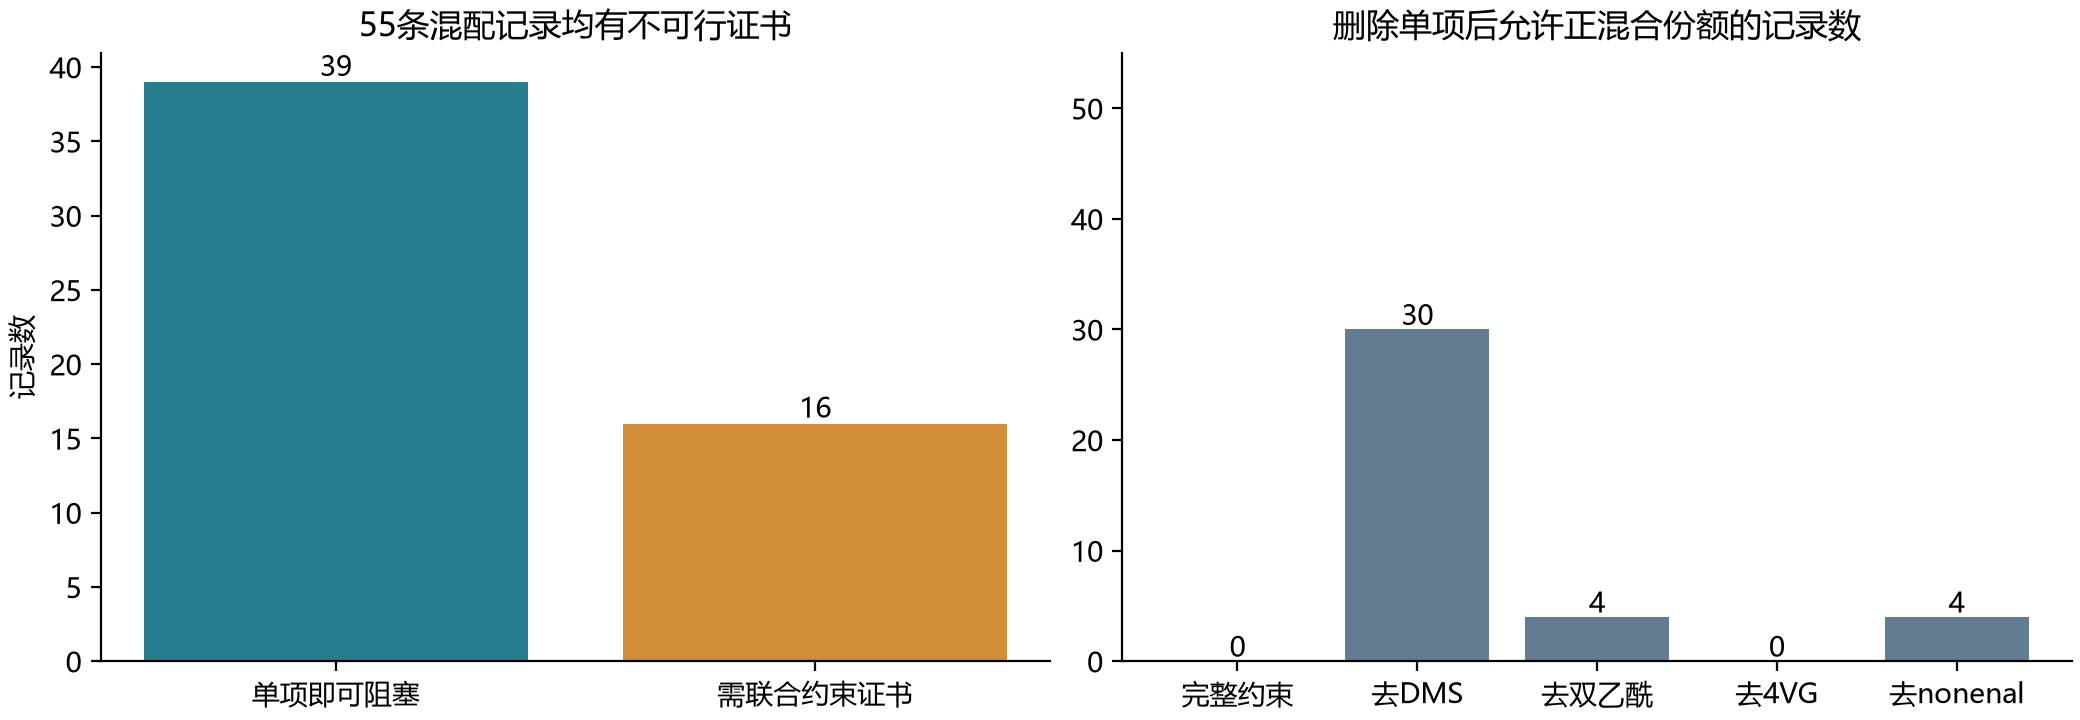
\includegraphics[width=0.95\textwidth]{figures/mixture_certificate.png}
\caption{严格混配约束的不可行证书及单项约束消融。}
\end{figure*}
\section{验证范围与应用建议}

本文以现有250款酒及历史面板为基础，按酒划分评价新酒预测；评分人员在训练与测试之间存在重叠。后续可采用人员留出设计，评价模型对新面板的适用性。对于非零等级，可继续比较两阶段模型及训练内部校准方法，并按目标和风格报告混淆矩阵与等级距离误差。


基于全部可用历史酒样，已拟合并保存最终均分融合模型与七级分布模型，模型文件包含预处理器、231个输入字段顺序、目标定义及可核验的参考单位。预测入口只读取化合物文件，并输出50项面板均分、众数、中位数和七级概率。三个历史酒样的无标签文件在独立目录完成流程检查；预测能力仍以按酒留出实验评价，并需由队员在新环境复跑。


实物验证可先将候选转化为具有批号的可制备小试，对四项化合物进行重复测量并记录检出限、定量限和回收率，再采用随机编码、平衡顺序的配对盲评。一个可执行的试验方案为30名训练人员、3个独立批次；以人员为单位汇总批次差异，对五项缺陷预先设定评价界限。新批次化学测量、盲评结果和制备条件将决定统计候选能否用于实际配方。


\section{结论}

基于公开逐人评分与附件样本核查，本文构造了50项0—6分面板均分和七级评分分布。固定融合模型在核心30项上的均分MAE为0.50222，较风格中位数基线低0.00747分；等级分布预测优于总体分布基线，但非零众数一致率为24.33\%，仍有明显提升空间。


化合物图对预测误差的影响随汇总口径变化，最终Top-3由普通岭模型产生。150条因素记录中36条满足描述性支持条件；结合风格内置换和化学文献，可以区分稳定关联与依赖风格结构的候选。


条件生成模型能够产生各目标风格的统计谱，独立代理复核显示迁移结果对评价模型敏感。严格浓度不增加约束下，55条记录均无正的Tripel混合份额；阈值超额风险约束下，参考阈值允许其中30条记录获得正份额。下一步应在同一冻结候选上联合检查风格、五项缺陷与制备条件，并通过新批次测量和盲评确认实际效果。


本文的数据核查、分析实现和文字整理使用了OpenAI Codex辅助；工具使用详情与队员实际复核记录另行提供。


\section*{参考文献}
\addcontentsline{toc}{section}{参考文献}
\noindent [1] Schreurs M, Piampongsant S, Roncoroni M, et al. Predicting and improving complex beer flavor through machine learning. Nature Communications, 15:2368, 2024. DOI:10.1038/s41467-024-46346-0.\par
\noindent [2] Schreurs M, et al. Data from: Predicting and improving complex beer flavor through machine learning, Version v4. Zenodo, 2026. \url{https://zenodo.org/records/23624915}，访问日期：2026年10月25日. DOI:10.5281/zenodo.23624915.\par
\noindent [3] Geurts P, Ernst D, Wehenkel L. Extremely randomized trees. Machine Learning, 63:3–42, 2006.\par
\noindent [4] Friedman J H. Greedy function approximation: A gradient boosting machine. The Annals of Statistics, 29(5):1189–1232, 2001.\par
\noindent [5] Breiman L. Stacked Regressions. Machine Learning, 24:49–64, 1996.\par
\noindent [6] Li C, Li H. Variable selection and regression analysis for graph-structured covariates with an application to genomics. The Annals of Applied Statistics, 4(3):1498–1516, 2010.\par
\noindent [7] Lei J, G'Sell M, Rinaldo A, et al. Distribution-Free Predictive Inference for Regression. Journal of the American Statistical Association, 113(523):1094–1111, 2018.\par
\noindent [8] Gneiting T, Raftery A E. Strictly Proper Scoring Rules, Prediction, and Estimation. Journal of the American Statistical Association, 102(477):359–378, 2007.\par
\noindent [9] Vanbeneden N, Saison D, Delvaux F, Delvaux F R. Decrease of 4-vinylguaiacol during beer aging and formation of apocynol and vanillin in beer. Journal of Agricultural and Food Chemistry, 56(24):11983–11988, 2008.\par
\noindent [10] Omur-Ozbek P, Dietrich A M, Duncan S E, Lee Y. Role of lipid oxidation, chelating agents, and antioxidants in metallic flavor development in the oral cavity. Journal of Agricultural and Food Chemistry, 60(9):2274–2280, 2012.\par
\noindent [11] Pater A, Satora P, Januszek M. Effect of Coriander Seed Addition at Different Stages of Brewing on Selected Parameters of Low-Alcohol Wheat Beers. Molecules, 29(4):844, 2024.\par
\noindent [12] Gretton A, Borgwardt K M, Rasch M J, et al. A Kernel Two-Sample Test. Journal of Machine Learning Research, 13:723–773, 2012.\par
\noindent [13] Meilgaard M C. Individual differences in sensory threshold for aroma chemicals added to beer. Food Quality and Preference, 4(3):153–167, 1993.\par
\noindent [14] Santos J R, et al. Determination of E-2-nonenal by high-performance liquid chromatography with UV detection assay for the evaluation of beer ageing. Journal of Chromatography A, 985(1–2):395–402, 2003.\par
\appendix
\section{全部50项Top-3与结果索引}


以下为原始面板均分的最终描述模型Top-3，括号为固定全数据参数条件下的200次bootstrap入选频率。$\lambda$=0，实际为普通岭回归；不是因果概率、独立检验p值或新化学试验。


\par\noindent{\scriptsize
\begin{tabular}{>{\raggedright\arraybackslash}p{0.425\columnwidth}>{\raggedright\arraybackslash}p{0.425\columnwidth}}
\toprule
目标 & Top-3字段（条件入选频率） \\
\midrule
A\_\allowbreak{}malt\_\allowbreak{}all & X2.\allowbreak{}acetylfuran (0.\allowbreak{}77)；ethyl.\allowbreak{}furoate (0.\allowbreak{}42)；phenethyl\_\allowbreak{}alcohol (0.\allowbreak{}36) \\
A\_\allowbreak{}malt\_\allowbreak{}grain & gamma.\allowbreak{}nonalactone (0.\allowbreak{}30)；car.\allowbreak{}3.\allowbreak{}en.\allowbreak{}2.\allowbreak{}one (0.\allowbreak{}36)；X5.\allowbreak{}methylfurfural (0.\allowbreak{}20) \\
A\_\allowbreak{}malt\_\allowbreak{}bread & furfural (0.\allowbreak{}36)；ethyl.\allowbreak{}furoate (0.\allowbreak{}28)；ethyl.\allowbreak{}tiglate (0.\allowbreak{}13) \\
A\_\allowbreak{}malt\_\allowbreak{}cara & X2.\allowbreak{}acetylfuran (0.\allowbreak{}60)；phenethyl\_\allowbreak{}alcohol (0.\allowbreak{}45)；octyl\_\allowbreak{}acetate (0.\allowbreak{}31) \\
\bottomrule
\end{tabular}}\par\smallskip
\par\noindent{\scriptsize
\begin{tabular}{>{\raggedright\arraybackslash}p{0.425\columnwidth}>{\raggedright\arraybackslash}p{0.425\columnwidth}}
\toprule
目标 & Top-3字段（条件入选频率） \\
\midrule
A\_\allowbreak{}malt\_\allowbreak{}burn & methylpyrazine (0.\allowbreak{}75)；X2.\allowbreak{}acetylfuran (0.\allowbreak{}60)；X4.\allowbreak{}methyl.\allowbreak{}1.\allowbreak{}pentanol (0.\allowbreak{}11) \\
A\_\allowbreak{}hops\_\allowbreak{}all & iron (0.\allowbreak{}56)；DMS (0.\allowbreak{}34)；cis.\allowbreak{}dihydro.\allowbreak{}beta.\allowbreak{}terpineol (0.\allowbreak{}20) \\
A\_\allowbreak{}hops\_\allowbreak{}citrus & X6.\allowbreak{}methyl.\allowbreak{}5.\allowbreak{}hepten.\allowbreak{}2.\allowbreak{}one (0.\allowbreak{}53)；terpinolene (0.\allowbreak{}19)；geraniol (0.\allowbreak{}26) \\
A\_\allowbreak{}hops\_\allowbreak{}tropical & DMS (0.\allowbreak{}55)；beta.\allowbreak{}phellandrene (0.\allowbreak{}26)；citronellol (0.\allowbreak{}29) \\
\bottomrule
\end{tabular}}\par\smallskip
\par\noindent{\scriptsize
\begin{tabular}{>{\raggedright\arraybackslash}p{0.425\columnwidth}>{\raggedright\arraybackslash}p{0.425\columnwidth}}
\toprule
目标 & Top-3字段（条件入选频率） \\
\midrule
A\_\allowbreak{}hops\_\allowbreak{}noble & iron (0.\allowbreak{}36)；ethyl\_\allowbreak{}octanoate (0.\allowbreak{}23)；ethyl\_\allowbreak{}decanoate (0.\allowbreak{}16) \\
A\_\allowbreak{}hops\_\allowbreak{}woody & iron (0.\allowbreak{}27)；ethyl\_\allowbreak{}2.\allowbreak{}methyl\_\allowbreak{}butyrate (0.\allowbreak{}15)；X2Z.\allowbreak{}6Z.\allowbreak{}farnesol (0.\allowbreak{}23) \\
A\_\allowbreak{}esters\_\allowbreak{}all & acetaldehyde (0.\allowbreak{}78)；X.\allowbreak{}E.\allowbreak{}.\allowbreak{}beta.\allowbreak{}ionone (0.\allowbreak{}23)；n.\allowbreak{}hexanol (0.\allowbreak{}23) \\
A\_\allowbreak{}esters\_\allowbreak{}ethac & acetaldehyde (0.\allowbreak{}40)；ethyl\_\allowbreak{}acetate (0.\allowbreak{}21)；cis.\allowbreak{}linalool.\allowbreak{}oxide (0.\allowbreak{}17) \\
\bottomrule
\end{tabular}}\par\smallskip
\par\noindent{\scriptsize
\begin{tabular}{>{\raggedright\arraybackslash}p{0.425\columnwidth}>{\raggedright\arraybackslash}p{0.425\columnwidth}}
\toprule
目标 & Top-3字段（条件入选频率） \\
\midrule
A\_\allowbreak{}esters\_\allowbreak{}isoaa & n.\allowbreak{}hexanol (0.\allowbreak{}40)；ambroxide (0.\allowbreak{}46)；ethyl.\allowbreak{}hexadecanoate (0.\allowbreak{}20) \\
A\_\allowbreak{}esters\_\allowbreak{}flower & beta.\allowbreak{}phellandrene (0.\allowbreak{}56)；X.\allowbreak{}E.\allowbreak{}.\allowbreak{}alpha.\allowbreak{}ionone (0.\allowbreak{}40)；terpinolene (0.\allowbreak{}14) \\
A\_\allowbreak{}esters\_\allowbreak{}fruity & beta.\allowbreak{}phellandrene (0.\allowbreak{}86)；X1.\allowbreak{}10.\allowbreak{}di.\allowbreak{}epi.\allowbreak{}cubenol (0.\allowbreak{}18)；benzyl.\allowbreak{}alcohol (0.\allowbreak{}30) \\
F\_\allowbreak{}malt\_\allowbreak{}all & acetaldehyde (0.\allowbreak{}57)；X2.\allowbreak{}acetylfuran (0.\allowbreak{}47)；X.\allowbreak{}E.\allowbreak{}.\allowbreak{}alpha.\allowbreak{}ionone (0.\allowbreak{}44) \\
\bottomrule
\end{tabular}}\par\smallskip
\par\noindent{\scriptsize
\begin{tabular}{>{\raggedright\arraybackslash}p{0.425\columnwidth}>{\raggedright\arraybackslash}p{0.425\columnwidth}}
\toprule
目标 & Top-3字段（条件入选频率） \\
\midrule
F\_\allowbreak{}malt\_\allowbreak{}grain & X2.\allowbreak{}3.\allowbreak{}butanedione (0.\allowbreak{}49)；gamma.\allowbreak{}nonalactone (0.\allowbreak{}14)；X3.\allowbreak{}methyl.\allowbreak{}2.\allowbreak{}butenal (0.\allowbreak{}18) \\
F\_\allowbreak{}malt\_\allowbreak{}bread & acetaldehyde (0.\allowbreak{}26)；dehydroxy.\allowbreak{}cis.\allowbreak{}linalool.\allowbreak{}oxide (0.\allowbreak{}23)；caryophylla.\allowbreak{}4.\allowbreak{}12.\allowbreak{}.\allowbreak{}8.\allowbreak{}13.\allowbreak{}.\allowbreak{}dien.\allowbreak{}5.\allowbreak{}alpha.\allowbreak{}ol (0.\allowbreak{}15) \\
F\_\allowbreak{}malt\_\allowbreak{}cara & acetaldehyde (0.\allowbreak{}62)；ethyl.\allowbreak{}nicotinate (0.\allowbreak{}27)；isobutyl.\allowbreak{}hexanoate (0.\allowbreak{}23) \\
F\_\allowbreak{}malt\_\allowbreak{}burn & X2.\allowbreak{}acetylfuran (0.\allowbreak{}51)；methylpyrazine (0.\allowbreak{}57)；MeSH (0.\allowbreak{}25) \\
\bottomrule
\end{tabular}}\par\smallskip
\par\noindent{\scriptsize
\begin{tabular}{>{\raggedright\arraybackslash}p{0.425\columnwidth}>{\raggedright\arraybackslash}p{0.425\columnwidth}}
\toprule
目标 & Top-3字段（条件入选频率） \\
\midrule
F\_\allowbreak{}hops\_\allowbreak{}all & cis.\allowbreak{}dihydro.\allowbreak{}beta.\allowbreak{}terpineol (0.\allowbreak{}70)；iron (0.\allowbreak{}70)；ethyl\_\allowbreak{}isovalerate (0.\allowbreak{}40) \\
F\_\allowbreak{}hops\_\allowbreak{}citrus & geraniol (0.\allowbreak{}47)；citronellol (0.\allowbreak{}43)；cis.\allowbreak{}dihydro.\allowbreak{}beta.\allowbreak{}terpineol (0.\allowbreak{}41) \\
F\_\allowbreak{}hops\_\allowbreak{}tropical & X6.\allowbreak{}methyl.\allowbreak{}5.\allowbreak{}hepten.\allowbreak{}2.\allowbreak{}one (0.\allowbreak{}46)；DMS (0.\allowbreak{}24)；citronellol (0.\allowbreak{}27) \\
F\_\allowbreak{}hops\_\allowbreak{}noble & iron (0.\allowbreak{}68)；citronellol (0.\allowbreak{}23)；X14.\allowbreak{}hydroxy.\allowbreak{}alpha.\allowbreak{}humulene (0.\allowbreak{}30) \\
\bottomrule
\end{tabular}}\par\smallskip
\par\noindent{\scriptsize
\begin{tabular}{>{\raggedright\arraybackslash}p{0.425\columnwidth}>{\raggedright\arraybackslash}p{0.425\columnwidth}}
\toprule
目标 & Top-3字段（条件入选频率） \\
\midrule
F\_\allowbreak{}hops\_\allowbreak{}woody & manool (0.\allowbreak{}43)；cis.\allowbreak{}dihydro.\allowbreak{}beta.\allowbreak{}terpineol (0.\allowbreak{}28)；n.\allowbreak{}octanol (0.\allowbreak{}15) \\
F\_\allowbreak{}esters\_\allowbreak{}all & acetaldehyde (0.\allowbreak{}91)；ethyl\_\allowbreak{}isovalerate (0.\allowbreak{}34)；n.\allowbreak{}hexanol (0.\allowbreak{}27) \\
F\_\allowbreak{}esters\_\allowbreak{}ethac & acetaldehyde (0.\allowbreak{}51)；ethyl\_\allowbreak{}acetate (0.\allowbreak{}47)；n.\allowbreak{}tetradecanol (0.\allowbreak{}28) \\
F\_\allowbreak{}esters\_\allowbreak{}isoaa & n.\allowbreak{}hexanol (0.\allowbreak{}28)；ethyl\_\allowbreak{}decanoate (0.\allowbreak{}14)；acetaldehyde (0.\allowbreak{}12) \\
\bottomrule
\end{tabular}}\par\smallskip
\par\noindent{\scriptsize
\begin{tabular}{>{\raggedright\arraybackslash}p{0.425\columnwidth}>{\raggedright\arraybackslash}p{0.425\columnwidth}}
\toprule
目标 & Top-3字段（条件入选频率） \\
\midrule
F\_\allowbreak{}esters\_\allowbreak{}flower & beta.\allowbreak{}phellandrene (0.\allowbreak{}30)；eucalyptol (0.\allowbreak{}29)；terpinolene (0.\allowbreak{}13) \\
F\_\allowbreak{}esters\_\allowbreak{}fruity & beta.\allowbreak{}phellandrene (0.\allowbreak{}49)；X.\allowbreak{}E.\allowbreak{}.\allowbreak{}beta.\allowbreak{}ionone (0.\allowbreak{}38)；MeSH (0.\allowbreak{}17) \\
acidity & lactic\_\allowbreak{}acid.\allowbreak{}mg.\allowbreak{}L.\allowbreak{} (1.\allowbreak{}00)；acetic\_\allowbreak{}acid.\allowbreak{}g.\allowbreak{}L.\allowbreak{} (0.\allowbreak{}72)；X4.\allowbreak{}ethyl.\allowbreak{}guaiacol (0.\allowbreak{}12) \\
bitternes & iron (0.\allowbreak{}98)；cis.\allowbreak{}dihydro.\allowbreak{}beta.\allowbreak{}terpineol (0.\allowbreak{}63)；ethyl\_\allowbreak{}octanoate (0.\allowbreak{}48) \\
\bottomrule
\end{tabular}}\par\smallskip
\par\noindent{\scriptsize
\begin{tabular}{>{\raggedright\arraybackslash}p{0.425\columnwidth}>{\raggedright\arraybackslash}p{0.425\columnwidth}}
\toprule
目标 & Top-3字段（条件入选频率） \\
\midrule
sweetness & ethyl\_\allowbreak{}decanoate (0.\allowbreak{}81)；iron (0.\allowbreak{}52)；ethyl\_\allowbreak{}octanoate (0.\allowbreak{}28) \\
X4vg & X4VG (1.\allowbreak{}00)；delta.\allowbreak{}terpinyl.\allowbreak{}acetate (0.\allowbreak{}26)；ethyl\_\allowbreak{}isovalerate (0.\allowbreak{}22) \\
diacetyl & CS2 (0.\allowbreak{}21)；X.\allowbreak{}E.\allowbreak{}.\allowbreak{}beta.\allowbreak{}ionone (0.\allowbreak{}09)；octyl\_\allowbreak{}acetate (0.\allowbreak{}29) \\
dms & SO2.\allowbreak{}mg.\allowbreak{}L.\allowbreak{} (0.\allowbreak{}56)；caryophylla.\allowbreak{}4.\allowbreak{}12.\allowbreak{}.\allowbreak{}8.\allowbreak{}13.\allowbreak{}.\allowbreak{}dien.\allowbreak{}5.\allowbreak{}alpha.\allowbreak{}ol (0.\allowbreak{}18)；neryl.\allowbreak{}formate (0.\allowbreak{}17) \\
\bottomrule
\end{tabular}}\par\smallskip
\par\noindent{\scriptsize
\begin{tabular}{>{\raggedright\arraybackslash}p{0.425\columnwidth}>{\raggedright\arraybackslash}p{0.425\columnwidth}}
\toprule
目标 & Top-3字段（条件入选频率） \\
\midrule
metallic & iron (0.\allowbreak{}94)；ethyl\_\allowbreak{}isovalerate (0.\allowbreak{}46)；neryl.\allowbreak{}formate (0.\allowbreak{}20) \\
stale\_\allowbreak{}hops & X2.\allowbreak{}butyloctanoate (0.\allowbreak{}41)；iron (0.\allowbreak{}27)；X.\allowbreak{}E.\allowbreak{}.\allowbreak{}ortho.\allowbreak{}methoxy.\allowbreak{}cinnamaldehyde (0.\allowbreak{}21) \\
t2n & germacrene.\allowbreak{}D (0.\allowbreak{}58)；isopentyl.\allowbreak{}hexanoate (0.\allowbreak{}46)；X.\allowbreak{}Z.\allowbreak{}.\allowbreak{}dihydro.\allowbreak{}apofarnesal (0.\allowbreak{}18) \\
orange & X1.\allowbreak{}alpha.\allowbreak{}terpineol (0.\allowbreak{}73)；limonene (0.\allowbreak{}49)；linalool (0.\allowbreak{}38) \\
\bottomrule
\end{tabular}}\par\smallskip
\par\noindent{\scriptsize
\begin{tabular}{>{\raggedright\arraybackslash}p{0.425\columnwidth}>{\raggedright\arraybackslash}p{0.425\columnwidth}}
\toprule
目标 & Top-3字段（条件入选频率） \\
\midrule
coriander & x.\allowbreak{}methyl.\allowbreak{}1.\allowbreak{}octanol (0.\allowbreak{}57)；geraniol (0.\allowbreak{}55)；linalool (0.\allowbreak{}46) \\
clove & linalool (0.\allowbreak{}81)；limonene (0.\allowbreak{}67)；eucalyptol (0.\allowbreak{}48) \\
lactic & lactic\_\allowbreak{}acid.\allowbreak{}mg.\allowbreak{}L.\allowbreak{} (1.\allowbreak{}00)；acetic\_\allowbreak{}acid.\allowbreak{}g.\allowbreak{}L.\allowbreak{} (0.\allowbreak{}61)；ethyl.\allowbreak{}phenylacetate (0.\allowbreak{}28) \\
acetic & lactic\_\allowbreak{}acid.\allowbreak{}mg.\allowbreak{}L.\allowbreak{} (1.\allowbreak{}00)；acetic\_\allowbreak{}acid.\allowbreak{}g.\allowbreak{}L.\allowbreak{} (0.\allowbreak{}62)；DES (0.\allowbreak{}23) \\
\bottomrule
\end{tabular}}\par\smallskip
\par\noindent{\scriptsize
\begin{tabular}{>{\raggedright\arraybackslash}p{0.425\columnwidth}>{\raggedright\arraybackslash}p{0.425\columnwidth}}
\toprule
目标 & Top-3字段（条件入选频率） \\
\midrule
barnyard & X2.\allowbreak{}butyloctanoate (0.\allowbreak{}32)；gamma.\allowbreak{}eudesmol (0.\allowbreak{}27)；iron (0.\allowbreak{}23) \\
alcohol & acetaldehyde (0.\allowbreak{}83)；ethanol.\allowbreak{}.\allowbreak{}v.\allowbreak{}v.\allowbreak{} (0.\allowbreak{}82)；X3.\allowbreak{}methyl.\allowbreak{}2.\allowbreak{}hexanol (0.\allowbreak{}47) \\
aftertaste & glycerol (0.\allowbreak{}68)；ethyl\_\allowbreak{}isovalerate (0.\allowbreak{}62)；cis.\allowbreak{}dihydro.\allowbreak{}beta.\allowbreak{}terpineol (0.\allowbreak{}34) \\
body & glycerol (0.\allowbreak{}80)；acetaldehyde (0.\allowbreak{}68)；X3.\allowbreak{}methyl.\allowbreak{}2.\allowbreak{}hexanol (0.\allowbreak{}47) \\
\bottomrule
\end{tabular}}\par\smallskip
\par\noindent{\scriptsize
\begin{tabular}{>{\raggedright\arraybackslash}p{0.425\columnwidth}>{\raggedright\arraybackslash}p{0.425\columnwidth}}
\toprule
目标 & Top-3字段（条件入选频率） \\
\midrule
co2 & ethyl\_\allowbreak{}octanoate (0.\allowbreak{}62)；X3.\allowbreak{}methyl.\allowbreak{}2.\allowbreak{}hexanol (0.\allowbreak{}55)；ethyl\_\allowbreak{}hexanoate (0.\allowbreak{}34) \\
overall & ethyl\_\allowbreak{}acetate (0.\allowbreak{}49)；X2.\allowbreak{}butyloctanoate (0.\allowbreak{}34)；ethyl\_\allowbreak{}hexanoate (0.\allowbreak{}14) \\
\bottomrule
\end{tabular}}\par\smallskip

\par\noindent{\scriptsize
\begin{tabular}{>{\raggedright\arraybackslash}p{0.425\columnwidth}>{\raggedright\arraybackslash}p{0.425\columnwidth}}
\toprule
目录 & 保存内容 \\
\midrule
audit & 对应关系、0-6端点、人员重复、浓度例外、OAV与候选公式 \\
prediction & 15折均分预测、标定对照、区间、原始尺度普通岭敏感性 \\
ordinal & 真实七级分布、众数/中位数/均分取整、缺失压力与生成谱等级画像 \\
raw\_\allowbreak{}graph/q2 & 原始端点无图/真图/打乱图、跨拟合贡献、完整Top-3 \\
\bottomrule
\end{tabular}}\par\smallskip
\par\noindent{\scriptsize
\begin{tabular}{>{\raggedright\arraybackslash}p{0.425\columnwidth}>{\raggedright\arraybackslash}p{0.425\columnwidth}}
\toprule
目录 & 保存内容 \\
\midrule
transfer & 冻结候选复查、G/J原始均分画像、浓度混合、LP与候选锁 \\
protocol & 空白评分表与假设样本量；没有实际品评结果 \\
\bottomrule
\end{tabular}}\par\smallskip

命令：python scripts/fetch\_stage4\_sources.py；python run\_stage4.py all --data-dir <官方附件目录>；python scripts/stage4\_graph\_comparison.py --data-dir <官方附件目录>；python -m pytest -q；python scripts/verify\_stage4.py；python scripts/stage4\_figures.py；python scripts/prepare\_absolute\_paper.py；使用scripts/build\_revised\_pdf.py按paper\_content.json生成本稿。首次重建旧生成谱时须先运行stage3；脚本默认来源目录可由参数指定。


软件：Python 3.12及NumPy、pandas、SciPy、scikit-learn、NetworkX、Matplotlib、openpyxl；精确版本在requirements-lock.txt和各运行manifest中。PDF排版另用ReportLab、pypdf、pdfplumber和Pillow；无需声称外部依赖库源码属于本队。


\section{完整源程序}
\subsection*{src/\_\_init\_\_.py}
\lstinputlisting{sources/001___init__.py}
\subsection*{src/audit.py}
\lstinputlisting{sources/002_audit.py}
\subsection*{src/common.py}
\lstinputlisting{sources/003_common.py}
\subsection*{src/data.py}
\lstinputlisting{sources/004_data.py}
\subsection*{src/q1.py}
\lstinputlisting{sources/005_q1.py}
\subsection*{src/q2.py}
\lstinputlisting{sources/006_q2.py}
\subsection*{src/q3.py}
\lstinputlisting{sources/007_q3.py}
\subsection*{src/reporting.py}
\lstinputlisting{sources/008_reporting.py}
\subsection*{src/stage2.py}
\lstinputlisting{sources/009_stage2.py}
\subsection*{src/stage3\_algorithms.py}
\lstinputlisting{sources/010_stage3_algorithms.py}
\subsection*{src/stage3\_generation.py}
\lstinputlisting{sources/011_stage3_generation.py}
\subsection*{src/stage3\_graph.py}
\lstinputlisting{sources/012_stage3_graph.py}
\subsection*{src/stage3\_prediction.py}
\lstinputlisting{sources/013_stage3_prediction.py}
\subsection*{src/stage4\_audit.py}
\lstinputlisting{sources/014_stage4_audit.py}
\subsection*{src/stage4\_models.py}
\lstinputlisting{sources/015_stage4_models.py}
\subsection*{src/stage4\_trial.py}
\lstinputlisting{sources/016_stage4_trial.py}
\subsection*{scripts/analyze\_trial.py}
\lstinputlisting{sources/017_analyze_trial.py}
\subsection*{scripts/build\_paper\_pdf.py}
\lstinputlisting{sources/018_build_paper_pdf.py}
\subsection*{scripts/build\_revised\_pdf.py}
\lstinputlisting{sources/019_build_revised_pdf.py}
\subsection*{scripts/fetch\_stage4\_sources.py}
\lstinputlisting{sources/020_fetch_stage4_sources.py}
\subsection*{scripts/package\_reference.py}
\lstinputlisting{sources/021_package_reference.py}
\subsection*{scripts/prepare\_absolute\_paper.py}
\lstinputlisting{sources/022_prepare_absolute_paper.py}
\subsection*{scripts/prepare\_paper.py}
\lstinputlisting{sources/023_prepare_paper.py}
\subsection*{scripts/prepare\_revised\_paper.py}
\lstinputlisting{sources/024_prepare_revised_paper.py}
\subsection*{scripts/prepare\_trial\_protocol.py}
\lstinputlisting{sources/025_prepare_trial_protocol.py}
\subsection*{scripts/render\_equations.py}
\lstinputlisting{sources/026_render_equations.py}
\subsection*{scripts/revised\_equations.py}
\lstinputlisting{sources/027_revised_equations.py}
\subsection*{scripts/stage2\_figures.py}
\lstinputlisting{sources/028_stage2_figures.py}
\subsection*{scripts/stage3\_figures.py}
\lstinputlisting{sources/029_stage3_figures.py}
\subsection*{scripts/stage3\_preflight.py}
\lstinputlisting{sources/030_stage3_preflight.py}
\subsection*{scripts/stage4\_figures.py}
\lstinputlisting{sources/031_stage4_figures.py}
\subsection*{scripts/stage4\_graph\_comparison.py}
\lstinputlisting{sources/032_stage4_graph_comparison.py}
\subsection*{scripts/verify\_absolute\_paper.py}
\lstinputlisting{sources/033_verify_absolute_paper.py}
\subsection*{scripts/verify\_reference.py}
\lstinputlisting{sources/034_verify_reference.py}
\subsection*{scripts/verify\_revised\_paper.py}
\lstinputlisting{sources/035_verify_revised_paper.py}
\subsection*{scripts/verify\_stage3.py}
\lstinputlisting{sources/036_verify_stage3.py}
\subsection*{scripts/verify\_stage4.py}
\lstinputlisting{sources/037_verify_stage4.py}
\subsection*{tests/test\_invariants.py}
\lstinputlisting{sources/038_test_invariants.py}
\subsection*{tests/test\_stage2.py}
\lstinputlisting{sources/039_test_stage2.py}
\subsection*{tests/test\_stage3\_algorithms.py}
\lstinputlisting{sources/040_test_stage3_algorithms.py}
\subsection*{tests/test\_stage3\_research.py}
\lstinputlisting{sources/041_test_stage3_research.py}
\subsection*{tests/test\_stage4.py}
\lstinputlisting{sources/042_test_stage4.py}
\subsection*{run.py}
\lstinputlisting{sources/043_run.py}
\subsection*{run\_stage2.py}
\lstinputlisting{sources/044_run_stage2.py}
\subsection*{run\_stage3.py}
\lstinputlisting{sources/045_run_stage3.py}
\subsection*{run\_stage4.py}
\lstinputlisting{sources/046_run_stage4.py}
\subsection*{config.json}
\lstinputlisting{sources/047_config.json}
\subsection*{config\_stage2.json}
\lstinputlisting{sources/048_config_stage2.json}
\subsection*{config\_stage3.json}
\lstinputlisting{sources/049_config_stage3.json}
\subsection*{config\_stage3\_design.json}
\lstinputlisting{sources/050_config_stage3_design.json}
\subsection*{config\_stage4.json}
\lstinputlisting{sources/051_config_stage4.json}
\subsection*{scripts/review\_experiments.py}
\lstinputlisting{sources/052_review_experiments.py}
\subsection*{src/review\_diagnostics.py}
\lstinputlisting{sources/053_review_diagnostics.py}
\subsection*{scripts/build\_latex\_revision.py}
\lstinputlisting{sources/054_build_latex_revision.py}
\subsection*{run\_final\_model.py}
\lstinputlisting{sources/055_run_final_model.py}
\subsection*{src/deployment.py}
\lstinputlisting{sources/056_deployment.py}
\subsection*{scripts/diagnose\_stage4.py}
\lstinputlisting{sources/057_diagnose_stage4.py}
\subsection*{tests/test\_deployment.py}
\lstinputlisting{sources/058_test_deployment.py}
\subsection*{scripts/ordinal\_two\_stage\_experiment.py}
\lstinputlisting{sources/059_ordinal_two_stage_experiment.py}
\subsection*{scripts/summarize\_two\_stage.py}
\lstinputlisting{sources/060_summarize_two_stage.py}
\subsection*{论文排版主文件 main.tex}
\lstinputlisting{main.tex}
\subsection*{赛事适配文档类 mathorcup-journal.cls}
\lstinputlisting{mathorcup-journal.cls}
\end{document}
